% Created by tikzDevice version 0.10.1 on 2016-08-26 10:29:27
% !TEX encoding = UTF-8 Unicode
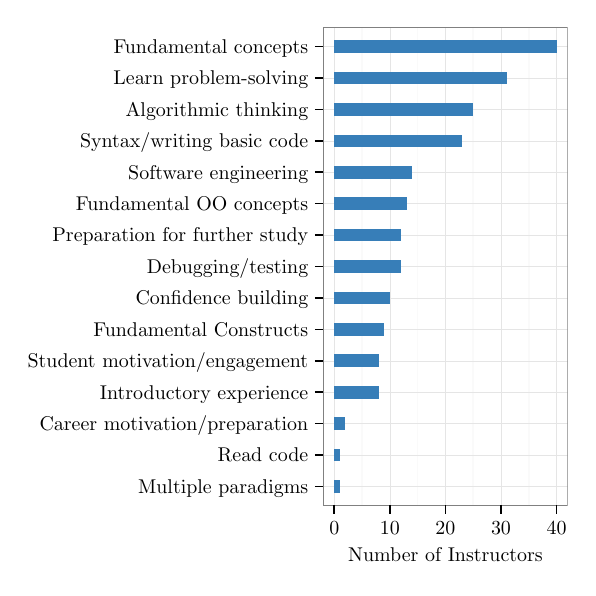
\begin{tikzpicture}[x=1pt,y=1pt]
\definecolor{fillColor}{RGB}{255,255,255}
\path[use as bounding box,fill=fillColor,fill opacity=0.00] (0,0) rectangle (195.13,195.13);
\begin{scope}
\path[clip] (  0.00,  0.00) rectangle (195.13,195.13);
\definecolor{drawColor}{RGB}{255,255,255}
\definecolor{fillColor}{RGB}{255,255,255}

\path[draw=drawColor,line width= 0.6pt,line join=round,line cap=round,fill=fillColor] (  0.00,  0.00) rectangle (195.13,195.13);
\end{scope}
\begin{scope}
\path[clip] (106.78, 22.52) rectangle (195.13,195.13);
\definecolor{fillColor}{RGB}{255,255,255}

\path[fill=fillColor] (106.78, 22.52) rectangle (195.13,195.13);
\definecolor{drawColor}{gray}{0.98}

\path[draw=drawColor,line width= 0.6pt,line join=round] (120.83, 22.52) --
	(120.83,195.13);

\path[draw=drawColor,line width= 0.6pt,line join=round] (140.91, 22.52) --
	(140.91,195.13);

\path[draw=drawColor,line width= 0.6pt,line join=round] (160.99, 22.52) --
	(160.99,195.13);

\path[draw=drawColor,line width= 0.6pt,line join=round] (181.07, 22.52) --
	(181.07,195.13);
\definecolor{drawColor}{gray}{0.90}

\path[draw=drawColor,line width= 0.2pt,line join=round] (106.78, 29.33) --
	(195.13, 29.33);

\path[draw=drawColor,line width= 0.2pt,line join=round] (106.78, 40.69) --
	(195.13, 40.69);

\path[draw=drawColor,line width= 0.2pt,line join=round] (106.78, 52.04) --
	(195.13, 52.04);

\path[draw=drawColor,line width= 0.2pt,line join=round] (106.78, 63.40) --
	(195.13, 63.40);

\path[draw=drawColor,line width= 0.2pt,line join=round] (106.78, 74.76) --
	(195.13, 74.76);

\path[draw=drawColor,line width= 0.2pt,line join=round] (106.78, 86.11) --
	(195.13, 86.11);

\path[draw=drawColor,line width= 0.2pt,line join=round] (106.78, 97.47) --
	(195.13, 97.47);

\path[draw=drawColor,line width= 0.2pt,line join=round] (106.78,108.82) --
	(195.13,108.82);

\path[draw=drawColor,line width= 0.2pt,line join=round] (106.78,120.18) --
	(195.13,120.18);

\path[draw=drawColor,line width= 0.2pt,line join=round] (106.78,131.54) --
	(195.13,131.54);

\path[draw=drawColor,line width= 0.2pt,line join=round] (106.78,142.89) --
	(195.13,142.89);

\path[draw=drawColor,line width= 0.2pt,line join=round] (106.78,154.25) --
	(195.13,154.25);

\path[draw=drawColor,line width= 0.2pt,line join=round] (106.78,165.60) --
	(195.13,165.60);

\path[draw=drawColor,line width= 0.2pt,line join=round] (106.78,176.96) --
	(195.13,176.96);

\path[draw=drawColor,line width= 0.2pt,line join=round] (106.78,188.32) --
	(195.13,188.32);

\path[draw=drawColor,line width= 0.2pt,line join=round] (110.79, 22.52) --
	(110.79,195.13);

\path[draw=drawColor,line width= 0.2pt,line join=round] (130.87, 22.52) --
	(130.87,195.13);

\path[draw=drawColor,line width= 0.2pt,line join=round] (150.95, 22.52) --
	(150.95,195.13);

\path[draw=drawColor,line width= 0.2pt,line join=round] (171.03, 22.52) --
	(171.03,195.13);

\path[draw=drawColor,line width= 0.2pt,line join=round] (191.11, 22.52) --
	(191.11,195.13);
\definecolor{fillColor}{RGB}{55,126,184}

\path[fill=fillColor] (110.79, 27.06) rectangle (112.80, 31.60);

\path[fill=fillColor] (110.79, 38.42) rectangle (112.80, 42.96);

\path[fill=fillColor] (110.79, 49.77) rectangle (114.81, 54.31);

\path[fill=fillColor] (110.79, 61.13) rectangle (126.86, 65.67);

\path[fill=fillColor] (110.79, 72.48) rectangle (126.86, 77.03);

\path[fill=fillColor] (110.79, 83.84) rectangle (128.86, 88.38);

\path[fill=fillColor] (110.79, 95.20) rectangle (130.87, 99.74);

\path[fill=fillColor] (110.79,106.55) rectangle (134.89,111.09);

\path[fill=fillColor] (110.79,117.91) rectangle (134.89,122.45);

\path[fill=fillColor] (110.79,129.26) rectangle (136.90,133.81);

\path[fill=fillColor] (110.79,140.62) rectangle (138.90,145.16);

\path[fill=fillColor] (110.79,151.98) rectangle (156.98,156.52);

\path[fill=fillColor] (110.79,163.33) rectangle (160.99,167.87);

\path[fill=fillColor] (110.79,174.69) rectangle (173.04,179.23);

\path[fill=fillColor] (110.79,186.04) rectangle (191.11,190.59);
\definecolor{drawColor}{gray}{0.50}

\path[draw=drawColor,line width= 0.6pt,line join=round,line cap=round] (106.78, 22.52) rectangle (195.13,195.13);
\end{scope}
\begin{scope}
\path[clip] (  0.00,  0.00) rectangle (195.13,195.13);
\definecolor{drawColor}{RGB}{0,0,0}

\node[text=drawColor,anchor=base east,inner sep=0pt, outer sep=0pt, scale=  0.72] at (101.38, 26.85) {Multiple paradigms};

\node[text=drawColor,anchor=base east,inner sep=0pt, outer sep=0pt, scale=  0.72] at (101.38, 38.21) {Read code};

\node[text=drawColor,anchor=base east,inner sep=0pt, outer sep=0pt, scale=  0.72] at (101.38, 49.56) {Career motivation/preparation};

\node[text=drawColor,anchor=base east,inner sep=0pt, outer sep=0pt, scale=  0.72] at (101.38, 60.92) {Introductory experience};

\node[text=drawColor,anchor=base east,inner sep=0pt, outer sep=0pt, scale=  0.72] at (101.38, 72.28) {Student motivation/engagement};

\node[text=drawColor,anchor=base east,inner sep=0pt, outer sep=0pt, scale=  0.72] at (101.38, 83.63) {Fundamental Constructs};

\node[text=drawColor,anchor=base east,inner sep=0pt, outer sep=0pt, scale=  0.72] at (101.38, 94.99) {Confidence building};

\node[text=drawColor,anchor=base east,inner sep=0pt, outer sep=0pt, scale=  0.72] at (101.38,106.34) {Debugging/testing};

\node[text=drawColor,anchor=base east,inner sep=0pt, outer sep=0pt, scale=  0.72] at (101.38,117.70) {Preparation for further study};

\node[text=drawColor,anchor=base east,inner sep=0pt, outer sep=0pt, scale=  0.72] at (101.38,129.06) {Fundamental OO concepts};

\node[text=drawColor,anchor=base east,inner sep=0pt, outer sep=0pt, scale=  0.72] at (101.38,140.41) {Software engineering};

\node[text=drawColor,anchor=base east,inner sep=0pt, outer sep=0pt, scale=  0.72] at (101.38,151.77) {Syntax/writing basic code};

\node[text=drawColor,anchor=base east,inner sep=0pt, outer sep=0pt, scale=  0.72] at (101.38,163.12) {Algorithmic thinking};

\node[text=drawColor,anchor=base east,inner sep=0pt, outer sep=0pt, scale=  0.72] at (101.38,174.48) {Learn problem-solving};

\node[text=drawColor,anchor=base east,inner sep=0pt, outer sep=0pt, scale=  0.72] at (101.38,185.84) {Fundamental concepts};
\end{scope}
\begin{scope}
\path[clip] (  0.00,  0.00) rectangle (195.13,195.13);
\definecolor{drawColor}{RGB}{0,0,0}

\path[draw=drawColor,line width= 0.6pt,line join=round] (103.78, 29.33) --
	(106.78, 29.33);

\path[draw=drawColor,line width= 0.6pt,line join=round] (103.78, 40.69) --
	(106.78, 40.69);

\path[draw=drawColor,line width= 0.6pt,line join=round] (103.78, 52.04) --
	(106.78, 52.04);

\path[draw=drawColor,line width= 0.6pt,line join=round] (103.78, 63.40) --
	(106.78, 63.40);

\path[draw=drawColor,line width= 0.6pt,line join=round] (103.78, 74.76) --
	(106.78, 74.76);

\path[draw=drawColor,line width= 0.6pt,line join=round] (103.78, 86.11) --
	(106.78, 86.11);

\path[draw=drawColor,line width= 0.6pt,line join=round] (103.78, 97.47) --
	(106.78, 97.47);

\path[draw=drawColor,line width= 0.6pt,line join=round] (103.78,108.82) --
	(106.78,108.82);

\path[draw=drawColor,line width= 0.6pt,line join=round] (103.78,120.18) --
	(106.78,120.18);

\path[draw=drawColor,line width= 0.6pt,line join=round] (103.78,131.54) --
	(106.78,131.54);

\path[draw=drawColor,line width= 0.6pt,line join=round] (103.78,142.89) --
	(106.78,142.89);

\path[draw=drawColor,line width= 0.6pt,line join=round] (103.78,154.25) --
	(106.78,154.25);

\path[draw=drawColor,line width= 0.6pt,line join=round] (103.78,165.60) --
	(106.78,165.60);

\path[draw=drawColor,line width= 0.6pt,line join=round] (103.78,176.96) --
	(106.78,176.96);

\path[draw=drawColor,line width= 0.6pt,line join=round] (103.78,188.32) --
	(106.78,188.32);
\end{scope}
\begin{scope}
\path[clip] (  0.00,  0.00) rectangle (195.13,195.13);
\definecolor{drawColor}{RGB}{0,0,0}

\path[draw=drawColor,line width= 0.6pt,line join=round] (110.79, 19.52) --
	(110.79, 22.52);

\path[draw=drawColor,line width= 0.6pt,line join=round] (130.87, 19.52) --
	(130.87, 22.52);

\path[draw=drawColor,line width= 0.6pt,line join=round] (150.95, 19.52) --
	(150.95, 22.52);

\path[draw=drawColor,line width= 0.6pt,line join=round] (171.03, 19.52) --
	(171.03, 22.52);

\path[draw=drawColor,line width= 0.6pt,line join=round] (191.11, 19.52) --
	(191.11, 22.52);
\end{scope}
\begin{scope}
\path[clip] (  0.00,  0.00) rectangle (195.13,195.13);
\definecolor{drawColor}{RGB}{0,0,0}

\node[text=drawColor,anchor=base,inner sep=0pt, outer sep=0pt, scale=  0.72] at (110.79, 12.16) {0};

\node[text=drawColor,anchor=base,inner sep=0pt, outer sep=0pt, scale=  0.72] at (130.87, 12.16) {10};

\node[text=drawColor,anchor=base,inner sep=0pt, outer sep=0pt, scale=  0.72] at (150.95, 12.16) {20};

\node[text=drawColor,anchor=base,inner sep=0pt, outer sep=0pt, scale=  0.72] at (171.03, 12.16) {30};

\node[text=drawColor,anchor=base,inner sep=0pt, outer sep=0pt, scale=  0.72] at (191.11, 12.16) {40};
\end{scope}
\begin{scope}
\path[clip] (  0.00,  0.00) rectangle (195.13,195.13);
\definecolor{drawColor}{RGB}{0,0,0}

\node[text=drawColor,anchor=base,inner sep=0pt, outer sep=0pt, scale=  0.72] at (150.95,  2.40) {Number of Instructors};
\end{scope}
\end{tikzpicture}
